\chapter{Basic concepts}
\label{chapter:epipilar_geo}

\section{Homogenous coordinate system}

In a projective geometry, homogenous coordinate system is used in the same way as Cartesian coordinates are used in Euclidian geometry. 
To transform a point $x=(u, v)$ from cartesian coordinates to homogenous, simply add the third coordinate 1: $x=(u, v, 1)$.
Homogenous coordinates are used to simplify the 2D transformation operations:

\begin{center}
    \textbf{Scale}
\end{center}
$$
\begin{bmatrix}
    x_1 \\ y_1
\end{bmatrix} = 
\begin{bmatrix}
    s_x & 0 \\
    0 & s_y
\end{bmatrix}
\begin{bmatrix}
    x_0 \\ y_0
\end{bmatrix}
$$ 
\begin{center}
    \textbf{Rotation}    
\end{center}
$$
\begin{bmatrix}
    x_1 \\ y_1
\end{bmatrix} = 
\begin{bmatrix}
    cos(\theta) & -sin(\theta) \\
    sin(\theta) & cos(\theta)
\end{bmatrix}
\begin{bmatrix}
    x_0 \\ y_0
\end{bmatrix}
$$
\begin{center}
    \textbf{Translation}    
\end{center}
$$
\begin{bmatrix}
    x_1 \\ y_1
\end{bmatrix} = 
\begin{bmatrix}
    x_0 \\ y_0
\end{bmatrix} +
\begin{bmatrix}
    t_x \\ t_y
\end{bmatrix}
$$ 

To aply any transformation we need to make a sequence of matrix multiplications, but this is not the case with translation - we need an addition operation for that. Here is how all this operations looks like in a projective geometry:

\begin{center}
    \textbf{Scale}
\end{center}
$$
\begin{bmatrix}
    x_1 \\ y_1 \\ 1
\end{bmatrix} = 
\begin{bmatrix}
    s_x & 0 & 0\\
    0 & s_y & 0\\
    0 & 0 & 1
\end{bmatrix}
\begin{bmatrix}
    x_0 \\ y_0 \\ 1
\end{bmatrix}
$$ 
\begin{center}
    \textbf{Rotation}    
\end{center}
$$
\begin{bmatrix}
    x_1 \\ y_1 \\ 1
\end{bmatrix} = 
\begin{bmatrix}
    cos(\theta) & -sin(\theta) & 0 \\
    sin(\theta) & cos(\theta)  & 0 \\
    0 & 0 & 1
\end{bmatrix}
\begin{bmatrix}
    x_0 \\ y_0 \\ 1
\end{bmatrix}
$$
\begin{center}
    \textbf{Translation}    
\end{center}
$$
\begin{bmatrix}
    x_1 \\ y_1 \\ 1
\end{bmatrix} = 
\begin{bmatrix}
    1 & 0 & t_x\\
    0 & 1 & t_y\\
    0 & 0 & 1
\end{bmatrix}
\begin{bmatrix}
    x_0 \\ y_0 \\ 1
\end{bmatrix}
$$ 

So in homogenous coordinate system all 2d tansformations can be combined and expressed as matrix multiplications.

\subsection{Infinity}
In Euclidian geometry parallel lines are the lines that have no intersection point. In projective geometry, parallel lines are intersecting in a point $x$ at infinity, $x = (u, v, 0)$. How is it possible?

\section{Pinhole camera model}
Pinhole camera - or a canonical perspective camera model - is a model of a simple camera without optics.
The very first example is a camera obscura - a dark room with a small hole, through which the image from outside is projected on the oposite wall. 
This model can be used to express camera geometry with field of view angles less than $180^{\circ}$.

\subsection{Camera coordinate system}
\begin{figure}[h]
    \centering
    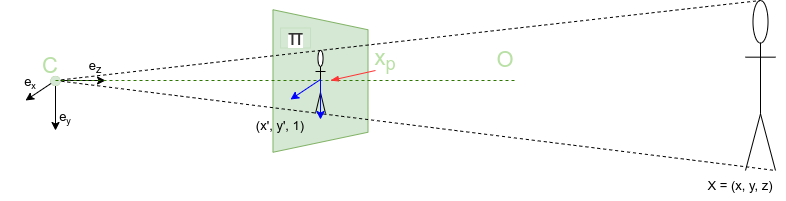
\includegraphics[width=1\textwidth]{graphics/td_scene.png}
    \caption{The pinhole camera model working scheme}
    \label{fig:td_scene_3d}
\end{figure}

\begin{figure}[h]
    \centering
    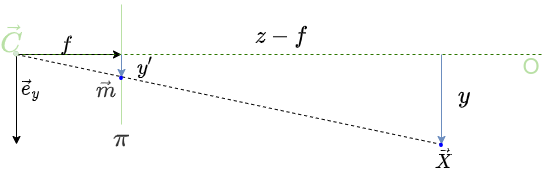
\includegraphics[width=1\textwidth]{graphics/td_scene_yz.png}
    \caption{The pinhole camera model, y-z plane}
    \label{fig:td_scene_yz}
\end{figure}

\begin{figure}[h]
    \centering
    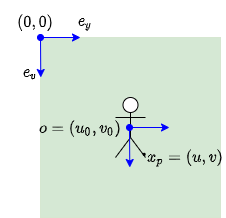
\includegraphics[width=.5\textwidth]{graphics/td_scene_xy.png}
    \caption{The pinhole camera model, x-y plane}
    \label{fig:td_scene_xy}
\end{figure}

In physical implementation of Obscure camera the projective plane is on the oposite side from the Projection center (or Camera center $C$ in pinhole camera model), the image is reversed and mirrored, but in most computer vision literature authors assume that it is on the same side as object (see \autoref{fig:td_scene_3d}).
In \autoref{fig:td_scene_3d} we are looking through a camera with camera center $C$ in a coordinate system with origin at $C$ and basis vectors $(e_x, e_y, e_z)$ on a human. 
Each point $X = (x, y, z)^T$ in a world coordinate system has it's projection $x_p = (x', y', 1)^T$ on a plane $\Pi$ which is located on a distance 1 from a camera center (\autoref{fig:td_scene_yz}). 
Optical axis $O$ is a ray perpendicular to plane $\Pi$, and on the image the point $ O \cap \Pi = x_p$ is a center of the image, see \autoref{fig:td_scene_xy}).

\subsection{Camera calibration matrix}
\begin{figure}[h]
    \centering
    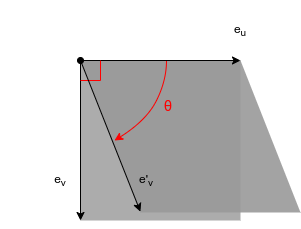
\includegraphics[width=.6\textwidth]{graphics/pixel.png}
    \caption{Scheme of pixel, changing the image (inner) reference frame}
    \label{fig:Kframes}
\end{figure}
Camera calibration matrix - a matrix that includes camera \textit{intrinsic} parameters - pixel size ($e_u$ and $e_v$) and pixel skew angle ($\theta$), as on \autoref{fig:Kframes}, pixel aspect ratio $\bf{a}$ and principle point coordinates $x_p = (u_0, v_0)$.
$$
K = \begin{bmatrix}
    af & -a f cot(\theta) & u_0 \\
    0 & f / sin(\theta) & v_0 \\
    0 & 0 & 1 \\
\end{bmatrix} \hspace{1cm} units: [f]=px, [u_0]=px, [v_0]=px, [a]=1
$$ 
Where $f$ is a focal length used to convert world length ratios to pixels.

In a modern world, every digital camera has a calibration matrix with a square pixel, so in most cases camera matrix looks like:

$$
K = \begin{bmatrix}
    f & 0 & u_0 \\
    0 & f & v_0 \\
    0 & 0 & 1 \\
\end{bmatrix}
$$

\subsection{Projection matrix}
\label{projection_matrix}
\begin{figure}[h]
    \centering
    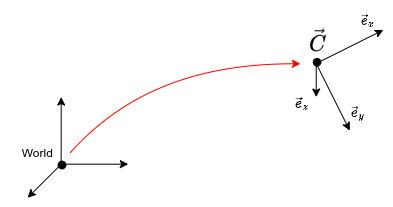
\includegraphics[width=.5\textwidth]{graphics/frames.png}
    \caption{Changing the world (outer) reference frame}
    \label{fig:frames}
\end{figure}
To translate a point from a world coordinate frame to image coordinate frame, Image projection matrix $P$ is used. 
The canonical projection matrix $P_0$ assumes that the camera is in the world coordinate center and that the calibration matrix $K = \bf{I}$
$$
P_0 = \begin{bmatrix} \bf{I} & | & 0 \end{bmatrix} = 
    \begin{bmatrix}
    1 & 0 & 0 & 0 \\
    0 & 1 & 0 & 0 \\
    0 & 0 & 1 & 0 \\
    \end{bmatrix}
$$
But this case is degenerate. 
As far as each camera is different, canonical projection matrix is never used, instead image projection matrix $P$ is used, with applied calibration matrix $K$ to transform canonical $P_0$ to perspective $P$:

$$
P = \bf{K} \begin{bmatrix} \bf{I} & | & 0 \end{bmatrix} = 
    \begin{bmatrix} 
    f & 0 & u_0 & 0 \\
    0 & f & v_0 & 0 \\ 
    0 & 0 & 1 & 0 \\
    \end{bmatrix}
$$

But not always the world coordinate center is located at point $C$ \autoref{fig:frames}. 
Usually it is rotated using a rotation matrix $R$ and translated on vector $t$ where $R$ is a $3x3$ matrix with $det(R) = 1$ and $R^{-1} = R^T$. 
So in general case:

$$
P =   K \begin{bmatrix} \bf{R} & | & \vec{\bf{t}} \end{bmatrix} = 
        K \begin{bmatrix} \bf{R} & | & - \bf{R} \bf{C} \end{bmatrix}
$$
where $C$ is quite often used as a camera position in a world reference frame. 
So matrix $P$ has 6 intrinsic parameters: 3 Euler angles and 3 translation components. 

\subsection{Projection equation}

Image point $m = (u, v)^T$ can be obtained from a point $X$ using $P$ 

$$
\lambda \begin{bmatrix} 
    u \\ v \\ 1 \end{bmatrix} = P \begin{bmatrix} x \\ y \\ z \\ 1
\end{bmatrix}
$$
$$
\lambda \begin{bmatrix} 
    \vec{m} \\ 1 \end{bmatrix} = P \begin{bmatrix} \vec{X} \\ 1
    \end{bmatrix}
$$
Where $\lambda \neq 0$
